% Latex header for doxygen 1.8.11
\documentclass[twoside]{book}

% Packages required by doxygen
\usepackage{fixltx2e}
\usepackage{calc}
\usepackage{doxygen}
\usepackage[export]{adjustbox} % also loads graphicx
\usepackage{graphicx}
\usepackage[utf8]{inputenc}
\usepackage{makeidx}
\usepackage{multicol}
\usepackage{multirow}
\PassOptionsToPackage{warn}{textcomp}
\usepackage{textcomp}
\usepackage[nointegrals]{wasysym}
\usepackage[table]{xcolor}

% Font selection
\usepackage[T1]{fontenc}
\usepackage[scaled=.90]{helvet}
\usepackage{courier}
\usepackage{amssymb}
\usepackage{sectsty}
\renewcommand{\familydefault}{\sfdefault}
\allsectionsfont{%
  \fontseries{bc}\selectfont%
  \color{darkgray}%
}
\renewcommand{\DoxyLabelFont}{%
  \fontseries{bc}\selectfont%
  \color{darkgray}%
}
\newcommand{\+}{\discretionary{\mbox{\scriptsize$\hookleftarrow$}}{}{}}

% Page & text layout
\usepackage{geometry}
\geometry{%
  a4paper,%
  top=2.5cm,%
  bottom=2.5cm,%
  left=2.5cm,%
  right=2.5cm%
}
\tolerance=750
\hfuzz=15pt
\hbadness=750
\setlength{\emergencystretch}{15pt}
\setlength{\parindent}{0cm}
\setlength{\parskip}{3ex plus 2ex minus 2ex}
\makeatletter
\renewcommand{\paragraph}{%
  \@startsection{paragraph}{4}{0ex}{-1.0ex}{1.0ex}{%
    \normalfont\normalsize\bfseries\SS@parafont%
  }%
}
\renewcommand{\subparagraph}{%
  \@startsection{subparagraph}{5}{0ex}{-1.0ex}{1.0ex}{%
    \normalfont\normalsize\bfseries\SS@subparafont%
  }%
}
\makeatother

% Headers & footers
\usepackage{fancyhdr}
\pagestyle{fancyplain}
\fancyhead[LE]{\fancyplain{}{\bfseries\thepage}}
\fancyhead[CE]{\fancyplain{}{}}
\fancyhead[RE]{\fancyplain{}{\bfseries\leftmark}}
\fancyhead[LO]{\fancyplain{}{\bfseries\rightmark}}
\fancyhead[CO]{\fancyplain{}{}}
\fancyhead[RO]{\fancyplain{}{\bfseries\thepage}}
\fancyfoot[LE]{\fancyplain{}{}}
\fancyfoot[CE]{\fancyplain{}{}}
\fancyfoot[RE]{\fancyplain{}{\bfseries\scriptsize Team 5572: The ROSBOTS }}
\fancyfoot[LO]{\fancyplain{}{\bfseries\scriptsize Team 5572: The ROSBOTS }}
\fancyfoot[CO]{\fancyplain{}{}}
\fancyfoot[RO]{\fancyplain{}{}}
\renewcommand{\footrulewidth}{0.4pt}
\renewcommand{\chaptermark}[1]{%
  \markboth{#1}{}%
}
\renewcommand{\sectionmark}[1]{%
  \markright{\thesection\ #1}%
}

% Indices & bibliography
\usepackage{natbib}
\usepackage[titles]{tocloft}
\setcounter{tocdepth}{3}
\setcounter{secnumdepth}{5}
\makeindex

% Hyperlinks (required, but should be loaded last)
\usepackage{ifpdf}
\ifpdf
  \usepackage[pdftex,pagebackref=true]{hyperref}
\else
  \usepackage[ps2pdf,pagebackref=true]{hyperref}
\fi
\hypersetup{%
  colorlinks=true,%
  linkcolor=blue,%
  citecolor=blue,%
  unicode%
}

% Custom commands
\newcommand{\clearemptydoublepage}{%
  \newpage{\pagestyle{empty}\cleardoublepage}%
}

\usepackage{caption}
\captionsetup{labelsep=space,justification=centering,font={bf},singlelinecheck=off,skip=4pt,position=top}

%===== C O N T E N T S =====

\begin{document}

% Titlepage & ToC
\hypersetup{pageanchor=false,
             bookmarksnumbered=true,
             pdfencoding=unicode
            }
\pagenumbering{roman}
\begin{titlepage}
\vspace*{7cm}
\begin{center}%
{\Large FRC 2018 Software Documentation}\\
\vspace*{1cm}
{\large Team 5572: The ROSBOTS}\\
\end{center}
\end{titlepage}
\clearemptydoublepage
\tableofcontents
\clearemptydoublepage
\pagenumbering{arabic}
\hypersetup{pageanchor=true}

%--- Begin generated contents ---
\chapter{Namespace Index}
\section{Namespace List}
Here is a list of all namespaces with brief descriptions\+:\begin{DoxyCompactList}
\item\contentsline{section}{\hyperlink{namespacedrivetrain}{drivetrain} }{\pageref{namespacedrivetrain}}{}
\item\contentsline{section}{\hyperlink{namespacemath}{math} }{\pageref{namespacemath}}{}
\end{DoxyCompactList}

\chapter{Class Index}
\section{Class List}
Here are the classes, structs, unions and interfaces with brief descriptions\+:\begin{DoxyCompactList}
\item\contentsline{section}{\hyperlink{classdrivetrain_1_1differential__drive}{drivetrain\+::differential\+\_\+drive} }{\pageref{classdrivetrain_1_1differential__drive}}{}
\item\contentsline{section}{\hyperlink{classdrivetrain_1_1motion__profile}{drivetrain\+::motion\+\_\+profile} }{\pageref{classdrivetrain_1_1motion__profile}}{}
\item\contentsline{section}{\hyperlink{structdrivetrain_1_1point}{drivetrain\+::point} }{\pageref{structdrivetrain_1_1point}}{}
\end{DoxyCompactList}

\chapter{File Index}
\section{File List}
Here is a list of all files with brief descriptions\+:\begin{DoxyCompactList}
\item\contentsline{section}{src/\hyperlink{drivetrain_8h}{drivetrain.\+h} }{\pageref{drivetrain_8h}}{}
\item\contentsline{section}{src/\hyperlink{test_8cpp}{test.\+cpp} }{\pageref{test_8cpp}}{}
\item\contentsline{section}{src/utils/\hyperlink{kernel__interface_8h}{kernel\+\_\+interface.\+h} }{\pageref{kernel__interface_8h}}{}
\item\contentsline{section}{src/utils/\hyperlink{linux_8cpp}{linux.\+cpp} }{\pageref{linux_8cpp}}{}
\item\contentsline{section}{src/utils/\hyperlink{matchdata_8h}{matchdata.\+h} }{\pageref{matchdata_8h}}{}
\end{DoxyCompactList}

\chapter{Namespace Documentation}
\hypertarget{namespacefield}{}\section{field Namespace Reference}
\label{namespacefield}\index{field@{field}}
\subsection*{Namespaces}
\begin{DoxyCompactItemize}
\item 
 \hyperlink{namespacefield_1_1side}{side}
\end{DoxyCompactItemize}

\hypertarget{namespacefield_1_1side}{}\section{field\+:\+:side Namespace Reference}
\label{namespacefield_1_1side}\index{field\+::side@{field\+::side}}
\subsection*{Functions}
\begin{DoxyCompactItemize}
\item 
void \hyperlink{namespacefield_1_1side_a776a4721046e56993639cb7ecf598b38}{setup} ()
\item 
bool \hyperlink{namespacefield_1_1side_a8d6d0f66b07887d59fd989ca7966eed6}{switch\+\_\+near} ()
\item 
bool \hyperlink{namespacefield_1_1side_a0d2e5824660082dc4eae6d2d838c64f5}{switch\+\_\+far} ()
\item 
bool \hyperlink{namespacefield_1_1side_a627d32e000cc5d518cbc61ceadf2e0d3}{scale} ()
\end{DoxyCompactItemize}
\subsection*{Variables}
\begin{DoxyCompactItemize}
\item 
const bool \hyperlink{namespacefield_1_1side_a7a93ec9e98b8a090cde3f064d3b97bfc}{left} = false
\item 
const bool \hyperlink{namespacefield_1_1side_a3fb1e4ea1c28a784c163ca4a8e17eef7}{right} = true
\end{DoxyCompactItemize}


\subsection{Function Documentation}
\index{field\+::side@{field\+::side}!scale@{scale}}
\index{scale@{scale}!field\+::side@{field\+::side}}
\subsubsection[{\texorpdfstring{scale()}{scale()}}]{\setlength{\rightskip}{0pt plus 5cm}bool field\+::side\+::scale (
\begin{DoxyParamCaption}
{}
\end{DoxyParamCaption}
)\hspace{0.3cm}{\ttfamily [inline]}}\hypertarget{namespacefield_1_1side_a627d32e000cc5d518cbc61ceadf2e0d3}{}\label{namespacefield_1_1side_a627d32e000cc5d518cbc61ceadf2e0d3}
\index{field\+::side@{field\+::side}!setup@{setup}}
\index{setup@{setup}!field\+::side@{field\+::side}}
\subsubsection[{\texorpdfstring{setup()}{setup()}}]{\setlength{\rightskip}{0pt plus 5cm}void field\+::side\+::setup (
\begin{DoxyParamCaption}
{}
\end{DoxyParamCaption}
)\hspace{0.3cm}{\ttfamily [inline]}}\hypertarget{namespacefield_1_1side_a776a4721046e56993639cb7ecf598b38}{}\label{namespacefield_1_1side_a776a4721046e56993639cb7ecf598b38}
\index{field\+::side@{field\+::side}!switch\+\_\+far@{switch\+\_\+far}}
\index{switch\+\_\+far@{switch\+\_\+far}!field\+::side@{field\+::side}}
\subsubsection[{\texorpdfstring{switch\+\_\+far()}{switch_far()}}]{\setlength{\rightskip}{0pt plus 5cm}bool field\+::side\+::switch\+\_\+far (
\begin{DoxyParamCaption}
{}
\end{DoxyParamCaption}
)\hspace{0.3cm}{\ttfamily [inline]}}\hypertarget{namespacefield_1_1side_a0d2e5824660082dc4eae6d2d838c64f5}{}\label{namespacefield_1_1side_a0d2e5824660082dc4eae6d2d838c64f5}
\index{field\+::side@{field\+::side}!switch\+\_\+near@{switch\+\_\+near}}
\index{switch\+\_\+near@{switch\+\_\+near}!field\+::side@{field\+::side}}
\subsubsection[{\texorpdfstring{switch\+\_\+near()}{switch_near()}}]{\setlength{\rightskip}{0pt plus 5cm}bool field\+::side\+::switch\+\_\+near (
\begin{DoxyParamCaption}
{}
\end{DoxyParamCaption}
)\hspace{0.3cm}{\ttfamily [inline]}}\hypertarget{namespacefield_1_1side_a8d6d0f66b07887d59fd989ca7966eed6}{}\label{namespacefield_1_1side_a8d6d0f66b07887d59fd989ca7966eed6}


\subsection{Variable Documentation}
\index{field\+::side@{field\+::side}!left@{left}}
\index{left@{left}!field\+::side@{field\+::side}}
\subsubsection[{\texorpdfstring{left}{left}}]{\setlength{\rightskip}{0pt plus 5cm}const bool field\+::side\+::left = false}\hypertarget{namespacefield_1_1side_a7a93ec9e98b8a090cde3f064d3b97bfc}{}\label{namespacefield_1_1side_a7a93ec9e98b8a090cde3f064d3b97bfc}
\index{field\+::side@{field\+::side}!right@{right}}
\index{right@{right}!field\+::side@{field\+::side}}
\subsubsection[{\texorpdfstring{right}{right}}]{\setlength{\rightskip}{0pt plus 5cm}const bool field\+::side\+::right = true}\hypertarget{namespacefield_1_1side_a3fb1e4ea1c28a784c163ca4a8e17eef7}{}\label{namespacefield_1_1side_a3fb1e4ea1c28a784c163ca4a8e17eef7}

\chapter{Class Documentation}
\hypertarget{structCurve}{}\section{Curve Struct Reference}
\label{structCurve}\index{Curve@{Curve}}


Describes the position and direction of a robot after a curve amount.  




{\ttfamily \#include $<$drivetrain.\+h$>$}

\subsection*{Public Attributes}
\begin{DoxyCompactItemize}
\item 
double \hyperlink{structCurve_a5d3af6bf8552bed573d4f3a1eeb70bd5}{x}
\begin{DoxyCompactList}\small\item\em Horizontal Position. \end{DoxyCompactList}\item 
double \hyperlink{structCurve_aabe742a202fc35bf2d30d24de017f62b}{y}
\begin{DoxyCompactList}\small\item\em Vertical Position. \end{DoxyCompactList}\item 
double \hyperlink{structCurve_a50248857e72a7f0dbfe1cdb55d2aca96}{heading}
\begin{DoxyCompactList}\small\item\em Direction of the robot in radians. \end{DoxyCompactList}\end{DoxyCompactItemize}


\subsection{Detailed Description}
Describes the position and direction of a robot after a curve amount. 

\subsection{Member Data Documentation}
\index{Curve@{Curve}!heading@{heading}}
\index{heading@{heading}!Curve@{Curve}}
\subsubsection[{\texorpdfstring{heading}{heading}}]{\setlength{\rightskip}{0pt plus 5cm}double Curve\+::heading}\hypertarget{structCurve_a50248857e72a7f0dbfe1cdb55d2aca96}{}\label{structCurve_a50248857e72a7f0dbfe1cdb55d2aca96}


Direction of the robot in radians. 

\index{Curve@{Curve}!x@{x}}
\index{x@{x}!Curve@{Curve}}
\subsubsection[{\texorpdfstring{x}{x}}]{\setlength{\rightskip}{0pt plus 5cm}double Curve\+::x}\hypertarget{structCurve_a5d3af6bf8552bed573d4f3a1eeb70bd5}{}\label{structCurve_a5d3af6bf8552bed573d4f3a1eeb70bd5}


Horizontal Position. 

\index{Curve@{Curve}!y@{y}}
\index{y@{y}!Curve@{Curve}}
\subsubsection[{\texorpdfstring{y}{y}}]{\setlength{\rightskip}{0pt plus 5cm}double Curve\+::y}\hypertarget{structCurve_aabe742a202fc35bf2d30d24de017f62b}{}\label{structCurve_aabe742a202fc35bf2d30d24de017f62b}


Vertical Position. 



The documentation for this struct was generated from the following file\+:\begin{DoxyCompactItemize}
\item 
src/\hyperlink{drivetrain_8h}{drivetrain.\+h}\end{DoxyCompactItemize}

\hypertarget{structDoublePair}{}\section{Double\+Pair Struct Reference}
\label{structDoublePair}\index{Double\+Pair@{Double\+Pair}}


Stores generic 2-\/value real number objects.  




{\ttfamily \#include $<$drivetrain.\+h$>$}

\subsection*{Public Attributes}
\begin{DoxyCompactItemize}
\item 
double \hyperlink{structDoublePair_a1a627a95488b8e575b162a37cc89b37e}{u}
\begin{DoxyCompactList}\small\item\em First Value. \end{DoxyCompactList}\item 
double \hyperlink{structDoublePair_ac04c81233ea3873cc9a790864a07735c}{v}
\begin{DoxyCompactList}\small\item\em Second Value. \end{DoxyCompactList}\end{DoxyCompactItemize}


\subsection{Detailed Description}
Stores generic 2-\/value real number objects. 

Examples of usage are 2d coordinates and differential drive outputs. 

\subsection{Member Data Documentation}
\index{Double\+Pair@{Double\+Pair}!u@{u}}
\index{u@{u}!Double\+Pair@{Double\+Pair}}
\subsubsection[{\texorpdfstring{u}{u}}]{\setlength{\rightskip}{0pt plus 5cm}double Double\+Pair\+::u}\hypertarget{structDoublePair_a1a627a95488b8e575b162a37cc89b37e}{}\label{structDoublePair_a1a627a95488b8e575b162a37cc89b37e}


First Value. 

\index{Double\+Pair@{Double\+Pair}!v@{v}}
\index{v@{v}!Double\+Pair@{Double\+Pair}}
\subsubsection[{\texorpdfstring{v}{v}}]{\setlength{\rightskip}{0pt plus 5cm}double Double\+Pair\+::v}\hypertarget{structDoublePair_ac04c81233ea3873cc9a790864a07735c}{}\label{structDoublePair_ac04c81233ea3873cc9a790864a07735c}


Second Value. 



The documentation for this struct was generated from the following file\+:\begin{DoxyCompactItemize}
\item 
src/\hyperlink{drivetrain_8h}{drivetrain.\+h}\end{DoxyCompactItemize}

\chapter{File Documentation}
\hypertarget{drivetrain_8h}{}\section{src/drivetrain/drivetrain.h File Reference}
\label{drivetrain_8h}\index{src/drivetrain/drivetrain.\+h@{src/drivetrain/drivetrain.\+h}}
{\ttfamily \#include $<$vector$>$}\\*
{\ttfamily \#include $<$utility$>$}\\*
{\ttfamily \#include \char`\"{}../util/math.\+h\char`\"{}}\\*
{\ttfamily \#include \char`\"{}W\+P\+I\+Lib.\+h\char`\"{}}\\*
Include dependency graph for drivetrain.\+h\+:

\hypertarget{test_8cpp}{}\section{src/test.cpp File Reference}
\label{test_8cpp}\index{src/test.\+cpp@{src/test.\+cpp}}
{\ttfamily \#include \char`\"{}utils/cpreprocessor.\+h\char`\"{}}\\*
{\ttfamily \#include \char`\"{}drivetrain.\+h\char`\"{}}\\*
{\ttfamily \#include $<$iostream$>$}\\*
Include dependency graph for test.\+cpp\+:\nopagebreak
\begin{figure}[H]
\begin{center}
\leavevmode
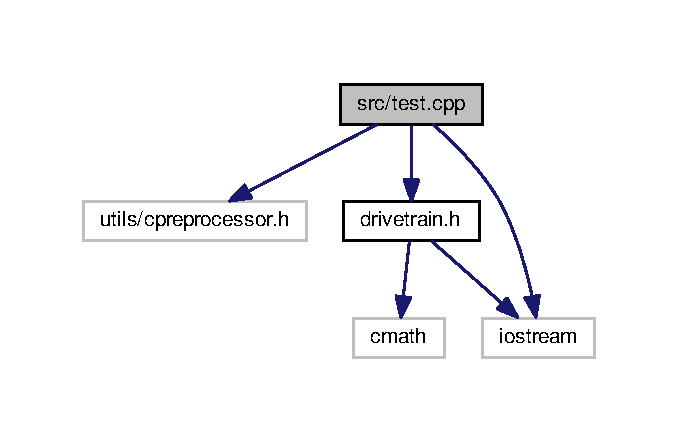
\includegraphics[width=326pt]{test_8cpp__incl}
\end{center}
\end{figure}
\subsection*{Functions}
\begin{DoxyCompactItemize}
\item 
int \hyperlink{test_8cpp_ae66f6b31b5ad750f1fe042a706a4e3d4}{main} ()
\end{DoxyCompactItemize}


\subsection{Function Documentation}
\index{test.\+cpp@{test.\+cpp}!main@{main}}
\index{main@{main}!test.\+cpp@{test.\+cpp}}
\subsubsection[{\texorpdfstring{main()}{main()}}]{\setlength{\rightskip}{0pt plus 5cm}int main (
\begin{DoxyParamCaption}
{}
\end{DoxyParamCaption}
)}\hypertarget{test_8cpp_ae66f6b31b5ad750f1fe042a706a4e3d4}{}\label{test_8cpp_ae66f6b31b5ad750f1fe042a706a4e3d4}

\hypertarget{matchdata_8h}{}\section{src/utils/matchdata.h File Reference}
\label{matchdata_8h}\index{src/utils/matchdata.\+h@{src/utils/matchdata.\+h}}
{\ttfamily \#include $<$string$>$}\\*
Include dependency graph for matchdata.\+h\+:\nopagebreak
\begin{figure}[H]
\begin{center}
\leavevmode
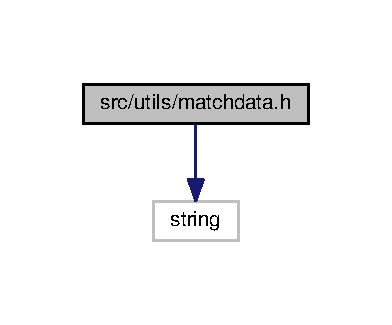
\includegraphics[width=188pt]{matchdata_8h__incl}
\end{center}
\end{figure}
\subsection*{Namespaces}
\begin{DoxyCompactItemize}
\item 
 \hyperlink{namespacefield}{field}
\item 
 \hyperlink{namespacefield_1_1side}{field\+::side}
\end{DoxyCompactItemize}
\subsection*{Functions}
\begin{DoxyCompactItemize}
\item 
void \hyperlink{namespacefield_1_1side_a776a4721046e56993639cb7ecf598b38}{field\+::side\+::setup} ()
\item 
bool \hyperlink{namespacefield_1_1side_a8d6d0f66b07887d59fd989ca7966eed6}{field\+::side\+::switch\+\_\+near} ()
\item 
bool \hyperlink{namespacefield_1_1side_a0d2e5824660082dc4eae6d2d838c64f5}{field\+::side\+::switch\+\_\+far} ()
\item 
bool \hyperlink{namespacefield_1_1side_a627d32e000cc5d518cbc61ceadf2e0d3}{field\+::side\+::scale} ()
\end{DoxyCompactItemize}
\subsection*{Variables}
\begin{DoxyCompactItemize}
\item 
const bool \hyperlink{namespacefield_1_1side_a7a93ec9e98b8a090cde3f064d3b97bfc}{field\+::side\+::left} = false
\item 
const bool \hyperlink{namespacefield_1_1side_a3fb1e4ea1c28a784c163ca4a8e17eef7}{field\+::side\+::right} = true
\end{DoxyCompactItemize}

%--- End generated contents ---

% Index
\backmatter
\newpage
\phantomsection
\clearemptydoublepage
\addcontentsline{toc}{chapter}{Index}
\printindex

\end{document}
